\documentclass[11pt,a4paper]{article}
\usepackage{graphicx}
\usepackage{pgfgantt}

\begin{document}
\title{Security Protocol for Courier-dependent Indirect Communication}
\author{Chen Sun}
\date{April 2014}
\maketitle

\section{Introduction}
In the modern world, Internet allows each pair of end-to-end nodes to build stable and reliable connections between them. However, in some extreme environments like interplanetary or under water, where stable and continuous connectivity can not be achieved, Internet may fail to provide its service. Entities in such environment can be abstracted as off-line entities as Internet is no longer available to them. \par 
One way to achieve communication between such off-line entities is using a portable device as courier to deliver the messages. Assuming there are two off-line entities Alice and Bob, and Alice wants to send Bob a message. What could happen is a portable device Courier (maybe several) copies the message from Alice, physically transported close to Bob and then delivers the message to Bob. Bearing such scenario in mind, this project is designated to design and implement a protocol to allow this kind of courier-dependent connection established efficiently and securely.\par 

\section{Background and Related Work}
Comparing to Internet which is relatively stable and reliable, so called challenged networks are characterized by latency, bandwidth limitations, error probability, node longevity, or path stability that are substantially worse than is typical of today's Internet \cite{fall}. To achieve successful communication within such networks, instead of using TCP/IP - which may serve disappointingly, each challenged network may has its own protocol. However, the diversity of these protocols prevents those networks to communicate with each other. The architecture of Delay-tolerant Network (DTN) was introduced to tackle the problem, achieving communication between various disparate challenged networks with significantly different sets of physical and operational constraints (latency, stability, etc.) \cite{burleigh} \cite{fall}. \par 
One of the key concept of DTN is custody transferring, which refers to the delivery of message from one DTN hop to another together with its reliable delivery responsibility. And using message couriers to achieve such custody transfer has been accepted as one practical implementation \cite{zhao}. Although the security issues of DTN have been discussed and evaluated in a high level \cite{cerf} \cite{symington} (mostly to prevent abuse of DTN), many concerns still remain to be considered in the specific courier-dependent message delivery scenario (like what if the courier could be hijacked and searched?). Referencing the high level security framework pre-defined, this project will dive into the detail of courier-dependent message delivery and create a practical security protocol for such scenario.



\section{Project Details}
\subsection{Project Overview}
As mentioned above, this project will focus on creating a security protocol for one of the implementations of custody transfer in Delay-Tolerant Network - courier-dependent message delivery. In this project, firstly a well-defined courier-dependent security communication protocol will be designed, then programs will be developed to implement such a protocol. After that, the developed programs will be tested and evaluated to show its practicality.

\subsection{Architecture and Environment}
\begin{figure}[h!]
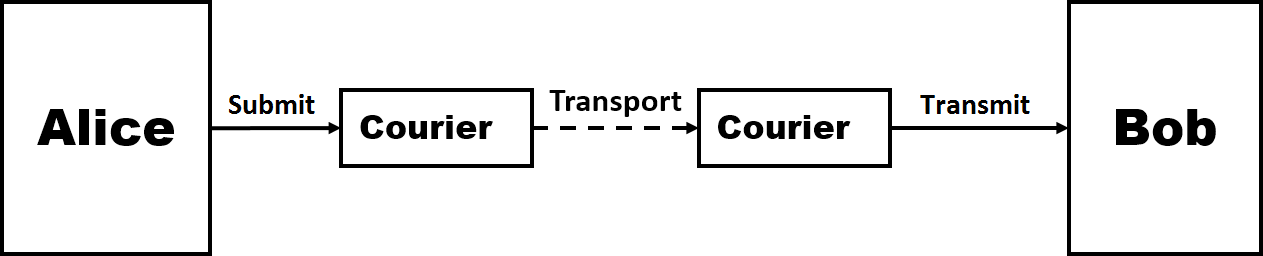
\includegraphics[width=\textwidth,natwidth=1263,natheight=256]{flowchart.png}
\caption{Simplified Scenario}
\end{figure}
To simplify the problem, we consider each message delivery independent to each other, as Figure 1 shows, a normal scenario of such independent delivery will be: Alice submits message to Courier, Courier physically transports to Bob, then finally transmits the message to Bob. Following this scenario, it separates the protocol into 2 different sub-protocols - submitting protocol and transmitting protocol, and both of them will be designed consistently in this project.\par
During the implementation phase, as off-line entities, Alice and Bob will be simulated by workstations (a laptop or desktop computer) while as portable devices, Courier will be simulated by mobile phones. So the implementation phase of this project will include programming for both computers and mobile phones.

\subsection{Potential Challenges}
The major challenge of this project is to come up with a practical security protocol for courier-dependent message delivery. According to the DTN architecture, some basic security requirements are indispensable \cite{cerf} and when applied to this specific scenario, those requirements can be interpreted into a more specific form. Following are the basic requirements of this project, based on the scenario that described in the former section:
\begin{itemize}
\item Authentication\\
As the cost of such communication will be high, it should abort delivery as soon as the unauthorized delivery quest is detected. So it requires any message delivered be authenticated by authorized entity (here Alice) and other entities are able to check the validity of it. 
\item Authenticity of Origin\\
The authenticity of origin of messages should be preserved during the communication, which means when Bob gets the message, he knows it must be Alice who create the message. It also implies the integrity of message is preserved.
\item Confidentiality of Message Content\\
The message content sent from Alice to Bob should be kept confidential to any entities except Alice and Bob. Because there is possibility that Courier could be hijacked and compromised, Courier should carry the data block without any knowledge of its actual content.
\item Reject Malicious Actions\\
Any malicious actions of Alice, Bob (like declare themselves as others or send message on behalf of others) or Courier (like change the content of the message it carries) will be detected and rejected, hopefully the compromised entity also will be caught and abandoned.
\end{itemize}
In addition, this project also has many variants to be considered as extensions:
\begin{itemize}
\item Efficiency concerns\\
Due to the potential limitation of computing and storage capability of Courier, and the high cost of such communication, protocol should be designed in such a way that it uses least number of messages and smallest message size to achieve the goal. Especially for cryptography, where overhead for encrypting/decrypting messages could be high, some measures should be used to reduce the overhead.
\item Key revocation\\
If one of the entities' key is disclosed, it must come up with a method for new keys to be securely revoked/exchanged. As in DTN a Key Distribute Centre would be extremely expensive to maintain, some new mechanisms should be introduced to reduce the cost of key revocation.
\item Deniable authentication\\
When Courier is hijacked and compromised by enemy during transporting, all messages exchanged before are considered exposed. In such situation, it would be plausible if Alice is able to deny the message that is already sent to Courier, which means enemy can not prove the origin of the message. This feature will be very important in military network or secret message delivery mission.
\item Courier-Courier Message Handover\\
Imagine the situation that a single message delivery is accomplished by only one Courier but several Couriers cooperatively: Courier$_1$ gets the message and handover it to Courier$_2$. Then the Courier$_2$ handover it to Courier$_3$. The handover could repeat several times and finally Courier$_n$ transmits the message to Bob. It requires a new sub-protocol to be defined and correspondingly the issues like authentication, confidentiality, deniable authentication, etc. should all be considered, which seems really tricky.
\end{itemize}

\subsection{Deliverables and Methodologies}
As mentioned before, this project mainly consists of 3 phases - protocol design, implementation and evaluation, each of them can be treated as a deliverable.

\subsubsection{Protocol Design}
In this phase a application-level communication protocol will be produced iteratively. As this protocol is designed for practical use, it should both meet the basic requirements and as many user scenarios as possible. Because there may be many potential factors to be considered in real user scenario (like does Courier have to be authenticated? or which entity be the initiator?), it requires the designing phase to be responsive and iterative as new stuff will keep being added during the phase.\par
As explained, the protocol may have several sub-protocols so at the end of designing phase, a full set of sub-protocols will be created together with their preconditions and postconditions to support specifying their user scenario.\par

\subsubsection{Protocol Implementation}
In the implementation phase programs implement the protocol will be developed in two parts - a core protocol library and the program that uses the core protocol library. The core library defines the abstract framework of the protocol and provides essential APIs for running it. It allows different implementations of the protocol to be developed in a consistent way.\par 
The program uses the core library is what can be actually run on a computer or mobile phone, to simulate the communication between entities. As the core library is just a framework, detail issues all lie on the implementation of the program. There will be many choices have to be considered and balanced - like connecting method, implementation of cryptography, message format, etc.. As the program efficiency will be evaluated in the third phase, the decisions have to be wisely made to make it as efficient as possible.\par 
Similar to any software engineering processes, the implementation phase consists of program designing, implementing and testing. And at the end of this phase, a set of self-contained programs will be developed running on computers and mobile phones which simulates Alice, Bob and Couriers respectively.

\subsubsection{Software Evaluating}
Finally the programs will be ran and evaluated by some of its critical features such as time efficiency, memory efficiency, scalability, etc.. \par 
Although the runnable program developed in this project will only be one specific implementation of all possible implementations and there must be better implementations than this, at least such evaluation shows ``the worst" behaviour of such protocol.

\subsection{Project Schedule}
At the beginning of the project, we can roughly separate the project into following parts:
\begin{enumerate}
\item Protocol Design
\item Software Development
\item Software Evalutation
\item Writting Thesis
\end{enumerate}
Figure 2 Gantt-Chart shows the draft time schedule for the whole project.

\begin{figure}[!h]
\hspace{-1.2in}
\begin{ganttchart}[
  hgrid,
  vgrid,
  x unit=0.8cm,
  y unit title=1.2cm,
  today=1,
  today rule/.style=%
  {ultra thick}
]{1}{18}
\gantttitle{April}{1} 
\gantttitle{May}{4} 
\gantttitle{June}{4} 
\gantttitle{July}{4} 
\gantttitle{Augest}{4} 
\gantttitle{Sep}{1} \\
\gantttitlelist{4}{1}
\gantttitlelist{1,...,4}{1}
\gantttitlelist{1,...,4}{1}
\gantttitlelist{1,...,4}{1}
\gantttitlelist{1,...,4}{1}
\gantttitlelist{1}{1} \\
\ganttbar{Protocol Design}{1}{2} \\
\ganttbar{Software Develop}{3}{12} \\
\ganttbar{Software Evaluate}{13}{14} \\
\ganttbar{Write Thesis}{15}{18}
\end{ganttchart}

\caption{Project Schedule}
\end{figure}


\section{Conclusion}
To sum up, first this proposal briefly explained the basic objective of this project - designing and implementing a security protocol for courier-dependent message delivery. Then some background of this project is given, showing the motivation. Basically this project discovers the security issues of one specific implementation of a part of Delay-Tolerant Network architecture and is inspired by some of the concerns DTN raises. After showing the background, some project details were revealed. The architecture of the aimed protocol is illustrated by graph first, and it mainly consists of two sub-protocols. Afterwards some major challenges of this project is listed, categorized as basic security requirements and extensions. Then 3 phases of the project - protocol design, protocol implementation and software evaluation, are explained briefly as its three primary deliverables. Finally the proposal split the project into number of reasonable steps and gave a estimated time schedule for undertaking each of them. 


\begin{thebibliography}{9}
\bibitem{burleigh}
  S. Burleigh, A. Hooke, L. Torgerson, K. Fall, V. Cerf, B. Durst, K. Scott and H. Weiss,
  \emph{Delay-Tolerant Networking: An Approach to Interplanetary Internet},
  IEEE Commun. Mag,
  pp. 128-136,
  June 2003.
 
\bibitem{cerf}
  V. Cerf, S. Burleigh, A. Hooke, L. Torgerson, R. Durst, K. Scott, K. Fall and H. Weiss,
  \emph{Delay-Tolerant Networking Architecture},
  IETF,
  RFC 4838,
  April 2007.
  [Online]. Available:http://tools.ietf.org/html/rfc4838

\bibitem{fall}
  K. Fall,
  \emph{A Delay-Tolerant Network Architecture for Challenged Internets},
  Proceedings SIGCOMM,
  Aug 2003.
  
\bibitem{symington}
  S. Symington, S. Farrell, H. Weiss,
  \emph{Bundle Security Protocol Specification},
  IRTF,
  RFC 6257,
  May 2011.
  [Online]. Available:http://www.rfc-base.org/txt/rfc-6257.txt

\bibitem{zhao}
  W. Zhao, M. Ammar and E. Zegura,
  \emph{Controlling the Mobility of Multiple Data Transport Ferries in a Delay-Tolerant Network},
  IEEE INFOCOM,
  2005.

\end{thebibliography}
\end{document}